\documentclass[tikz,dvisvgm]{standalone}
\usetikzlibrary{3d}

\begin{document}
    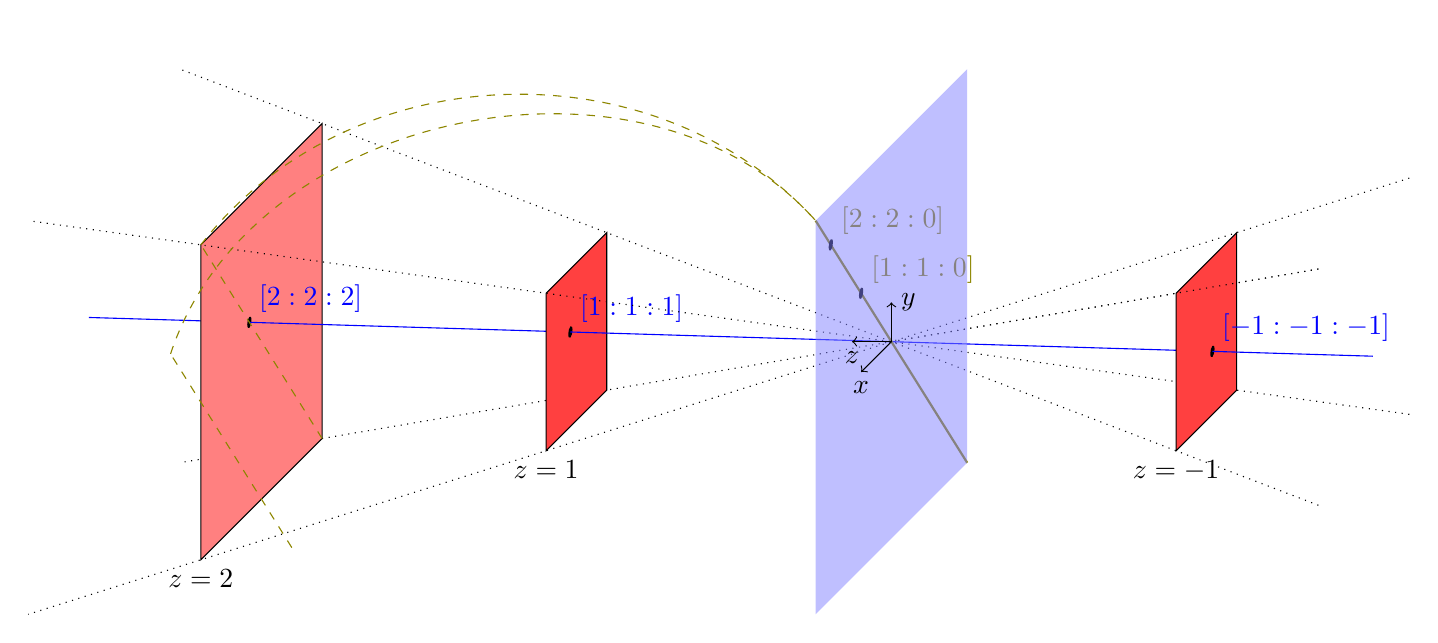
\begin{tikzpicture}

        \draw[dotted] (6,  1.5,  1.5) -- (0, 0, 0) -- (-8, -2, -2) -- (-10, -2.5, -2.5);
        \draw[dotted] (6, -1.5,  1.5) -- (0, 0, 0) -- (-8,  2, -2) -- (-10,  2.5, -2.5);
        \draw[blue] (-8, 0.4, 0.4) -- (-10, 0.5, 0.5);

        \begin{scope}[canvas is yz plane at x=-8]
            \filldraw[fill=red!50!white] (-2, -2) rectangle (2, 2);
            \fill[black] (0.4, 0.4) circle (2pt);
            \draw[blue] (0.4, 0.4) node [above right] {$[2:2:2]$};
        \end{scope}

        \draw[blue] (-4, 0.2, 0.2) -- (-8, 0.4, 0.4);

        \begin{scope}[canvas is yz plane at x=-4]
            \filldraw[fill=red!75!white] (-1, -1) rectangle (1, 1);
            \fill[black] (0.2, 0.2) circle (2pt);
            \draw[blue] (0.2, 0.2) node [above right] {$[1:1:1]$};
        \end{scope}

        \draw[dotted] (6,  1.5, -1.5) -- (0, 0, 0) -- (-8, -2,  2) -- (-10, -2.5,  2.5);
        \draw[dotted] (6, -1.5, -1.5) -- (0, 0, 0) -- (-8,  2,  2) -- (-10,  2.5,  2.5);
        \draw[blue] (4, -0.2, -0.2) -- (0, 0, 0) -- (-4, 0.2, 0.2);

        \begin{scope}[canvas is yz plane at x=4]
            \filldraw[fill=red!75!white] (-1, -1) rectangle (1, 1);
            \fill[black] (-0.2, -0.2) circle (2pt);
            \draw[blue] (-0.2, -0.2) node [above right] {$[-1:-1:-1]$};
        \end{scope}

        \draw[dotted] (6, 1.5, 1.5) -- (0, 0, 0);
        \draw[blue] (4, -0.2, -0.2) -- (6, -0.3, -0.3);

        \draw (-4, -1, 1) node [below] {$z=1$};
        \draw (-8, -2, 2) node [below] {$z=2$};
        \draw (4, -1, 1) node [below] {$z=-1$};

        \begin{scope}[canvas is yz plane at x=0]
            \draw[olive, thick] (-2.5, -2.5) -- 
                (1, 1) node [above right] {$[1:1:0]$} -- 
                (2, 2) node [above right] {$[2:2:0]$} -- (2.5, 2.5);
            \fill (1, 1) circle (2pt);
            \fill (2, 2) circle (2pt);
            \fill[blue!50!white, opacity=0.5] (-2.5, -2.5) rectangle (2.5, 2.5);
        \end{scope}

        \draw [->] (0, 0, 0) -- (0, 0, 1) node [below] {$x$};
        \draw [->] (0, 0, 0) -- (0, 0.5, 0) node [right] {$y$};
        \draw [->] (0, 0, 0) -- (-0.5, 0, 0) node [below] {$z$};

        \draw [olive, dashed] (-8, -2, -2) -- (-8, 2, 2);
        \draw [olive, dashed] (-8, -3, -1) -- (-8, 1, 3);
        \draw [olive, dashed] (-8, 2, 2) to [bend left = 50] (0, 2.5, 2.5);
        \draw [olive, dashed] (-8, 1, 3) to [bend left = 60] (0, 2.5, 2.5);
    \end{tikzpicture}
\end{document}
